
\chapter{Fundamentals of the Computational Methods} % Main chapter title

\label{Chapter3} % Change X to a consecutive number; for referencing this chapter elsewhere, use \ref{ChapterX}
\onehalfspace

\section{Molecular Dynamics}

\subsection{Background and Formalution}
Molecular Dynamics (MD) is a kind of molecular simulation that uses molecular configurations (Cartesian coordinates and momentum) to extract structural , thermodynamical and dynamical information of a system. This information is extracted from the time evolution of a syequationsstem, which are obtained  through the Newton motion  numerical integration \cite{tuckerman}:

\begin{equation}
\frac{d \vec{p}_{i}}{dt} = - \frac{\partial U (\vec{r}_{N})}{\partial \vec{r}_{i}}
\end{equation}
where $p_{i}$ is the momentum and $r^{N}$ are the coordinates of all the atoms$(x_{1},y_{1},z_{1},...,x_{N},y_{N},z_{N})$. Alternatively, we can write the equation relative to the velocity ($v_{i}$):
\begin{equation}
m_{i} \frac{\vec{v}_{i}}{dt} = - \frac{\partial U (\vec{r}_{N})}{\partial \vec{r}_{i}}
\end{equation}

In order to develop equations for any coordinate system ($q^{N}=(r_{1},\theta _{1},\phi _{1})$), the Halmitonian formulation, a more generalized formulation of classical mechanics,  is used to develop the equations of motion:
\begin{equation}
\mathcal{H} (q^{N},p^{N}) = K(p^{N}) + U(q^{N}) 
\end{equation}

In the equation above, $K$ is the kinetic energy and $U$ is the potential energy. The equations of motion can now be represented by:

\begin{equation}
\frac{d \vec{p}_{i}}{dt} = - \frac{\partial \mathcal{H}}{\partial \vec{q}_{i}}
\end{equation}

\begin{equation}
\frac{d \vec{q}_{i}}{dt} = - \frac{\partial \mathcal{H}}{\partial \vec{q}_{i}}
\end{equation}

The coordinates and momentum axes fo each atoms in a 6N dimensional space is defined as the phase space. The trajectory through the phase space is then the time evolution of a system in a molecular dynamics simulation. This evolution of the simulation may be then used to calculate the thermodynamic properties if the system is ergodic. That is, a trajectory in this system's will explore with the same probability all regions of the phase space of microstates with the same energy. 

\subsection{Statistical Ensembles}

A statistical ensemble corresponds to the set of configurations of a system with control variables defined. For a isolated system at equilibrium, the ensemble will correspond  to the microcanonical ensemble. The microcanonical ensemble have constant values of  number of particles (N), volume (V) and total energy (E). Following the ergodic hypothesis, the system at these conditions will then spend the same amount of time in each of the microstates (points in phase space) with the fixed E.  The number of accessible microstates is defined by the partition function or the density of states, and, for the microcanonical ensemble, is given by: 

\begin{equation}
\begin{aligned}
 \Omega (N,V,E) = \frac{1}{h^{3N}N!} \int dp^{N} dr^{N} \delta [\mathcal{H})(p^{N},r^{N}) -E]
\end{aligned}
\end{equation}
where h is the Planck constant and the delta functions is a Dirac delta function. As mentioned above, the system has equal probabilities an these can be written as:

\begin{equation}
\begin{aligned}
\varrho (p^{N},r^{N}) = \frac{[\mathcal{H})(p^{N},r^{N}) -E]}{ \Omega (N,V,E)} 
\end{aligned}
\end{equation}

The relation of the microcanonical partition function to the macroscopic entropy is:

\begin{equation}
\begin{aligned}
S = k_{b} ln \Omega (N,V,E) 
\end{aligned}
\end{equation}
where $k_{b}$ is the Boltzmann constant. Other properties can be derived form the equation using the fundamental equation or its energy version:

\begin{equation}
\begin{aligned}
dS = \frac{1}{T} dE + \frac{P}{T} dV + \frac{\mu}{T} dN
\end{aligned}
\end{equation}

\begin{equation}
\begin{aligned}
dE = T dS + P dV + \mu dN
\end{aligned}
\end{equation}

As said above, the microcanonical ensemble  have  N,V,E as its control variable. Other ensembles can also be defined according to the macroscopic properties held constant.  In the canonical ensemble,  N, V and the temperature (T) are held constant and  N, pressure (P) and T are held constant in the isothermal-isobaric ensemble. Other ensembles include the isenthalpic-isobaric (constant number of particles, pressure and enthalpy) and the grand canonical (constant chemical potential, volume and temperature). A variety of physical properties are measure at the conditions of the isenthalpic-isobaric ensemble such as enthalpies, entropies, redox potential, equilibrium constants and free energies, what makes this ensemble one of the most important \cite{tuckerman}. This is also the ensemble in which solvation free energy simulations are carried at this work, hence we going to briefly talk about it. This ensemble is obtained from a Legendre transformation on the canonical ensemble. The Helmholtz free energy $A(N,V,T)$ is becomes the Gibbs free energy $G(N,P,T)$ by transforming the volume into the external pressure:
\begin{equation}
G(N,P,T) = A(N,V(P),T) + PV(P)
\end{equation}


The Gibbs free energy is related to its the partition function $\Delta (N,P,T)$ (the number of accessible microstates) by:

\begin{equation}
\label{eq:fisobari}
\begin{aligned}
G(N,P,T) = -\kappa_{b}T ln \Delta (N,P,T)
\end{aligned}
\end{equation}

\begin{equation}
\label{eq:partiso}
\begin{aligned}
\Delta (N,P,T) = \frac{1}{V_{0}} \int_{0}^{\infty} dV \int d^{N}p d^{N}r \exp \left[ -\beta \left( \sum_{i=1}^{N}\dfrac{p_{i}^{2}}{2m_{i}} + U(r^{N}) + PV(r^{N}) \right) \right]
\end{aligned}
\end{equation}

where $Q (N,V,T)$ is the partition function of the canonical ensemble. From this relations and a differential change in G, we can obtain the chemical potential ($\mu$), volume and entropy ($S$) relations for this ensemble:

\begin{equation}
\mu = (\frac{\partial G}{\partial N})_{P,T} = - \kappa_{b} T (\frac{\partial ln \Delta (N,P,T)}{\partial N})_{N,T}
\end{equation}  
\begin{equation}
\langle V \rangle= (\frac{\partial G}{\partial P})_{N,T}= \kappa_{b} T (\frac{\partial ln \Delta (N,P,T)}{\partial N})_{N,P}
\end{equation}
\begin{equation}
S = (\frac{\partial G}{\partial T})_{N,P}= \kappa_{b}  (ln Q(N,V,T)+ T(\frac{\partial ln Q (N,V,T)}{\partial T})_{V,N})
\end{equation}

The isothermal-isobaric ensembles have external conditional been applied to it (temperature and pressure, respectively). For temperature control, the method employed  is to mimic the effect of a thermal reservoir through a thermostat. The most widely used thermostat are the Berendsen and Nosé-Hoover \cite{doi:10.1063/1.448118,PhysRevA.31.1695}. Meanwhile, the pressure is controlled with a barostat, that allows volume fluctuation. Among the more used barostats are the Berendsen, Hoover, Martina-Tobias-Klein and Parrinnello-Rahman \cite{doi:10.1063/1.448118,PhysRevA.31.1695,doi:10.1063/1.467468,doi:10.1063/1.328693}. It is possible to impose movements restrictions on the molecule or even consider the molecule as a rigid body in order to increase the integration step or to follow the modeling of the molecules. Methods for this include the SHAKE, RATTLE and Kamberaj algorithms \cite{RYCKAERT1977327,anderson1983,kamberaj}.

\subsection{Integration of the motion's equations}

With the formalism defined for the equations of motions an for the statistical ensemble, we can then derive discrete-time numerical approximations for them.  The basic idea is to solve the trajectory of atoms as function of time ($r^{N}(t)$) by updating the positions in discrete time intervals or time steps. One of the possible algorithms is The Verlet \cite{verlet}. Its proposed equation for the coordinates update is:  

\begin{equation}
r(t+ \Delta t) = 2r(t) - r(t+ \Delta t) + \frac{F(t)}{m} \Delta t^{2} +\vartheta (\Delta t^{4})
\end{equation}

In this equation, the positions are updated by a time step of $\Delta t$ by using the positions at the previous two time steps and the forces at $\Delta t$. The forces ($F$) acting on every particle are calculated by doing directional derivatives of the intermolecular potential $U(r)$, generally described by a force field, in relation to the atoms' positions:
\begin{equation}
\label{eq:forces}
\vec{F }(r)_{i} =  - \nabla U(r)
\end{equation}

The velocities of this method can be approximated by:

\begin{equation}
v(t+ \Delta t) = \frac{r(t+ \Delta t) - r(t- \Delta t)}{2 \Delta t} +\vartheta (\Delta t^{3})
\end{equation}

The Verlet method doesn't use the velocity directly to update the positions. Hence, the Velocity Verlet algorithm was proposed to serve as a reformulation of the Verlet algorithm that uses the velocity: 

\begin{equation}
r(t+ \Delta t) = r(t) +v(t) \Delta t + \frac{F(t)}{2m} \Delta t^{2}
\end{equation}

The velocity in the equation above is updated following:
\begin{equation}
v(t+ \Delta t) = v(t) +\frac{F(t+ \Delta t) +F(t)}{2m} \Delta t
\end{equation}

Instead of using a time step of $\Delta t$, the velocities can be updated at $\Delta t /2$. This is the strategy proposed by the leap frog algorithm:

\begin{equation}
v(t+ \Delta t /2) = v(t- \Delta t /2) +\frac{F(t+ \Delta t) +F(t)}{m} \Delta t
\end{equation}

\begin{equation}
r(t+ \Delta t) = r(t) +v(t+ \Delta t /2) \Delta t
\end{equation}

\subsection{Initial Configuration}

In order to use the equations above, every MD simulation need a non overlapping initial positions and velocities for every atom in the system. The initial velocities follow a temperature dependent Maxwell-Boltzmann distribution:

\begin{equation}
\varrho (v_{x,i}) = {\frac{m_{i}}{2 \pi k_{b} T}}^{\frac{1}{2}} exp(-\frac{m_{i}v_{x,i}^2}{2 \pi k_{b} T})
\end{equation}

Meanwhile, the initial positions are usually acquired by placing the molecules on a cubic lattice. The cubic lattice has a finite size, but  a finite size box would result in simulations dominated by surface effects. To avoid that, we can create a box periodically repeated in all directions by applying the so called Periodic Boundary Conditions (PBC). The periodic box has a primitive cell, which contains the system N particles, replicated in periodic lattice of infinite cells as represented in Figure \ref{fig:pbc}\cite{frenkel}.
\begin{figure*}
	\centering
	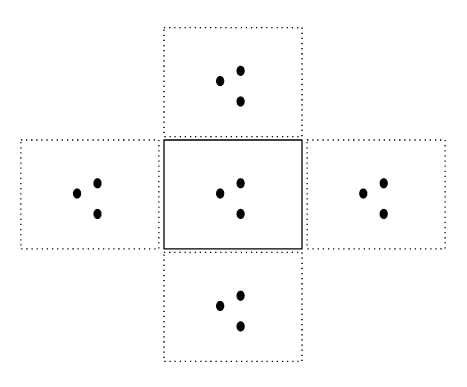
\includegraphics[width=0.7\textwidth]{Figures/pbc}
	\caption{Periodic boundary condition representation. Taken from \citeonline{frenkel}}
	\label{fig:pbc}
\end{figure*}
\FloatBarrier

\subsection{Force Fields }
Force fields are models for the description of structural characteristics such as van der Waals interactions, bond lengths, bond angles and torsion. The description is done by approximating the potential energy function ($U(r^N)$). $U(r^N)$ has contributions due to intermolecular and intramolecular interactions. The intramolecular interactions include bond stretching, bond angle bending and bond torsion. The contribution for the bond stretching is usually given by the following Taylor expansion around the energy minimum:

\begin{equation}
u_{bs}(d) = k_{bs} (d - d_{0})^2
\end{equation}

Here, $d$ is the bond length, $d_{0}$ is the equilibrium bond length and $k_{bs}$ is bond stretching constant. The bond angle bending contribution corresponds to deviations from the preferred geometry, and is given by:

\begin{equation}
u_{ab}(\theta) = k_{ab} (\theta - \theta _{0})^2
\end{equation}
where $k_{ab}$ and $\theta _{0}$ are constants defined by the force field and $\theta$ is the bond angle between three atoms.  The bond torsion interactions corresponds to the energies of rotations along bonds and it happens among four atoms:

\begin{equation}
u_{bt}(\omega) = \sum_{n=0}^{N}  c_{n} cos(\omega) ^{n}
\end{equation}
where N is the number of terms, $c_{n}$ is the summation index defined by the force field and $\omega$ is the torsional angle defined by the force field. 

The intermolecular interactions include electrostatics interactions, van der Waal interactions and volume repulsions. The electrostatics interactions of two atoms i and j with partial charges follow the Coulomb's Law:

\begin{equation}
u_{q}(r_{ij}) = \frac{q_{i}q_{j}}{4 \pi \epsilon _{0} r_{ij}}
\end{equation} 

In the equation above, $q_{i}$ and $q_{j}$ are the partial charges and  $\epsilon _{0}$ is the free space permittivity constant. In many force fields, the van der Waal interactions and volume repulsions between particles i and j are modeled in the same equation by the Lennard Jones Potential:
\begin{equation}
u_{LJ}(r_{ij}) = 4 \epsilon
\left[ \left(\frac{\sigma}{r} \right)^{12} - \left(\frac{\sigma}{r} \right)^{6} \right]
\end{equation}
where r is the distance the molecules, $\epsilon$ is the depth of the potential well, $\sigma$ is the distance correspondent to a zero intermolecular potential. The graphical representation of the potential is:
\begin{figure}[H]
	\centering
	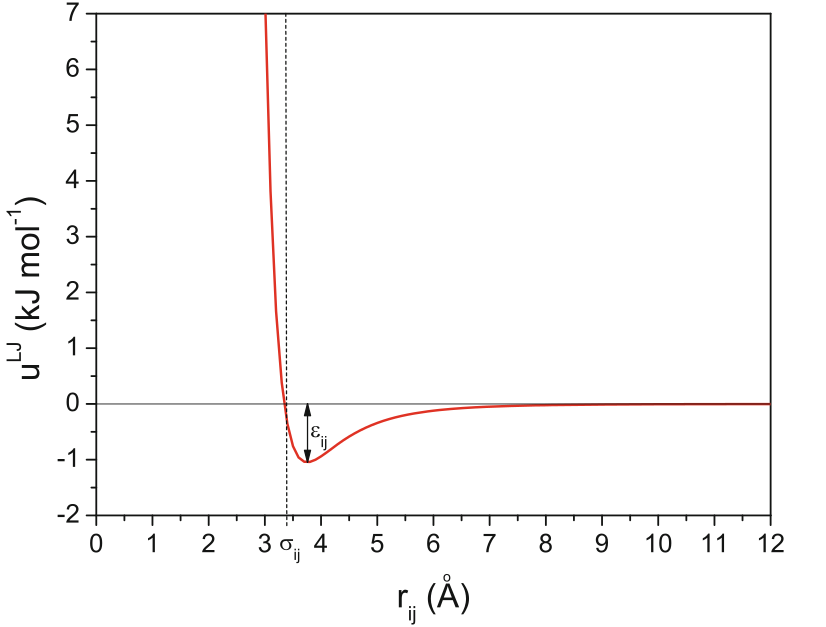
\includegraphics[width=0.8\linewidth]{Figures/lj2}
	\caption{Lennard Jones potential representation for two atoms of argon (i,j). Taken from \citeonline{raabe} }
	\label{fig:lj}
\end{figure}

The interactions in Figure \ref{fig:lj} tend to zero after a certain value of r, so this value can be set as the cutoff radius in which the potential energy is considered to be zero after it. Also, only interactions with te nearest periodic image of the cell is considered in order   for short range interactions (Minimum image convention condition). With this conditions, the calculations of forces and velocities are viable.

The final potential energy function defined by the force field can then be expressed by summing all the interactions above:

\begin{equation}
\begin{aligned}
U(r^N) = u_{bs}(d) + u_{ab}(\theta) + u_{bt}(\omega) + u_{q}(r_{ij}) + u_{LJ}(r_{ij})
\end{aligned}
\end{equation}
  
\section{SAFT-$\gamma$ Mie Force Field}


\subsection{SAFT-VR Mie EoS}

The SAFT-VR Mie equation of state \cite{lafitte2013} is the basis for the SAFT-$\gamma$ Mie coarse grained force field \cite{avendano2011}. This EoS was initially developed to describe chain molecule formed from fused Mie segments using the Mie attractive and repulsive potential. The Mie potential is a type of generalized Lennard-Jones potential that can be used to explicitly describe repulsive interactions of different hardness/softness and attractive interactions of different ranges, and is given by:
\begin{equation}
U_{Mie}(r) = \epsilon\frac{\lambda_r}{\lambda_r - \lambda_a} \left(\frac{\lambda_r}{\lambda_a} \right)^{\left( \frac{\lambda_a}{\lambda_r - \lambda_a} \right)}
\left[ \left(\frac{\sigma}{r} \right)^{\lambda_r} - \left(\frac{\sigma}{r} \right)^{\lambda_a} \right]
\label{eqn:miepotential}
\end{equation}
where $\lambda_r$ is the repulsive exponent and $\lambda_a$ is the attractive exponent. This equation uses the \citeonline{bh1976} high perturbation expansion of the Helmholtz free energy up to third order and an improved expression for the  radial distribution function (RDF) of Mie monomers at contact to obtain an equation able to give an accurate theoretical description of the vapor-liquid equilibrium and second derivative properties \cite{lafitte2013}. For a non-associating fluid, the Helmholtz free energy is:
\begin{equation}
\frac{A}{N\kappa_{b}T} = a = a^{IDEAL} + a^{MONO} + a^{CHAIN}
\label{eqn:miehelm}
\end{equation}

\subsubsection{Ideal Contribution}

The ideal contribution for a mixture is given by:
\begin{equation}
a^{IDEAL} = \sum_{i=1}^{N_{c}} x_{i}\ln{(\rho_{i}{\Lambda_{i}}^3)} -1
\label{eqn:aideal}
\end{equation}
where $x_{i}=N_{i}/N$ is the molar fraction of component i, $\rho_{i}=N_{i}/V$ is the number density, $N_{i}$ is the number of molecules of each component and $\Lambda_{i}^3$ is the de Broglie wavelength. 

\subsubsection{Monomer Contribution}

The monomer contribution describes interactions between Mie segments and can be expressed, for a mixture, as:
\begin{equation}
a^{MONO} = \left(\sum_{i=1}^{N_{c}} x_{i}m_{s,i} \right)a^{M}
\label{eqn:amonomer}
\end{equation}

In the equation above, $m_{s,i}$ is the number of spherical segments making up the molecule i and $a^{M}$  is the monomer dimensionless Helmholtz free energy and it is expressed as a third order perturbation expansion in the inverse temperature \cite{bh1976}:
\begin{equation}
a^{M} = a^{HS}+\beta{a_{1}}+\beta{a_{2}}^2+\beta{a_{3}}^3 
\label{eqn:aM}
\end{equation}
where $\beta=\kappa_{b}T$ and $a^{HS}$ is the hard-sphere dimensionless Helmholtz free energy for a mixture :
\begin{equation}
a^{HS} = \frac{6}{\pi\rho_{s}}\left[\left(\frac{\zeta^3_2}{\zeta^2_3}-\zeta_0 \right)\ln(1-\zeta_3)+\frac{3\zeta_{1}\zeta_{2}}{1-\zeta_3}+ \frac{\zeta^3_2}{\zeta_{3}(1-\zeta_3)^2}\right]
\label{eqn:hs}
\end{equation}

The variable $\rho_{s}=\rho\sum_{i}^{N_c} x_{i}m{s,i}$ is the total number density of spherical segments and $\zeta_l$ are the moments of the number density:
\begin{equation}
\zeta_l = \frac{\pi\rho_s}{6}\left(\sum_{i=1}^{N_c} x_{s,i}d^l_{ii} \right), l = 0,1,2,3
\label{eqn:zetal}
\end{equation}
where $x_{s,i}$ is the mole fraction of segments and is related through the mole fraction of component i ($x_i$) by:
\begin{equation}
x_{s,i} = \frac{m_{s,i}x_i}{\sum_{k=1}^{N_c} m_{s,k}x_{k} }
\label{eqn:xsi}
\end{equation}


The effective hard-sphere diameter $d_{ii}$ for the segments is:
\begin{equation}
d_{ii} =\int_{0}^{\sigma_{ii}} ( 1 - \exp(-\beta U^{Mie}_{ii}(r)) ) dr
\label{eqn:diameter}
\end{equation}


The integral in Eq. \eqref{eqn:diameter} is normally obtained by means of Gauss-Legendre with a 5-point quadrature \cite{papa2014}. The detailing of terms of Eq. \eqref{eqn:amonomer} can be found in \citeonline{lafitte2013}.

\subsubsection{Chain Contribution}
The chain formation of $m_{s}$ tangentially bonded Mie segments contribution is based on the first-order perturbation theory (TPT1)  \cite{papa2014} and can be expressed as:
\begin{equation}
a^{CHAIN} =-\sum_{i=1}^{N_{c}} x_{i}(m_{s,i} - 1)\ln(g_{ii}^{Mie}(\sigma_{ii}))
\label{eqn:achain}
\end{equation}


The $g_{ij}^{Mie}(\sigma_{ij})$ term correspond to the radial distribution function (RDF) of the hypothetical Mie system evaluated at the effective diameter and can be obtained with the perturbation expansion:
\begin{equation}
\begin{aligned}
g_{ij}^{Mie}(\sigma_{ij}) =g_{d,ij}^{HS}(\sigma_{ij})\exp[\beta\epsilon g_{1,ij}(\sigma_{ij})/g_{d,ij}^{HS}(\sigma_{ij}) + (\beta\epsilon)^{2} g_{2,ij}(\sigma_{ij})/g_{d,ij}^{HS}(\sigma_{ij})]
\end{aligned}
\label{eqn:gmie}
\end{equation}


The other terms in the equations above are explicitly exposed in the original article \cite{lafitte2013}. 

\subsubsection{Ring Contribution}
There are two forms for the Helmholtz free energy for rings formed from $m_{s}$ tangentially bonded segments in the literature. The first one  \cite{lafitte2012} considered that the difference between a chain and a ring molecule is that the latter has one more bond that is connecting the first segment to the last. With this assumption, Eq. \eqref{eqn:achain} can be adapted to rings by:
\begin{equation}
a^{RING} =-\sum_{i=1}^{N_{c}} x_{i}m_{s,i}\ln(g_{ii}^{Mie}(\sigma_{ii}))
\label{eqn:aringlafitte}
\end{equation}

According to \citeonline{lafitte2012}, Eq. \eqref{eqn:aringlafitte} needs an additional parameterization with molecular simulation data so the EoS can  be used in molecular simulations, but this procedure is not necessary for chain molecules. Recently, \citeonline{muller2017} tried to correct this inconsistency by means of developing the ring free energy based on the work of \citeonline{muller1993}, who obtained rigorous expressions for hard fluids with molecular geometries of rings of $m_s=3$. The final expression developed for the ring dimensionless Helmholtz free energy is:
\begin{equation}
a^{RING} =-\sum_{i=1}^{N_{c}} x_{i}(m_{s,i}-1+\chi_{i}\eta_{i})\ln(g_{ii}^{Mie}(\sigma_{ii}))
\label{eqn:aringmuller}
\end{equation}

$\eta_{i}=m_{s,i}\rho_{i}\sigma_{ii}^{3}/6$ is the packing fraction and $\chi_{i}$ is a parameter which depends on $m_{s,i}$ and on the geometry of the ring of each component i. For a value of $\chi=0$, Eq. \eqref{eqn:aringmuller} is equal to Eq. \eqref{eqn:achain}. Meanwhile, the equation corresponds to a hard sphere system of triangles when $\chi=1.3827$. \citeonline{muller2017} also calculated values of $\zeta$ for $m_{s}=3,m_{s}=4,m_{s}=5,m_{s}=7$ with pseudo-experimental data from molecular dynamics (MD) for a defined pure fluid. The values of $\chi$ for each geometry estimated can be seen in \figref{ringqsi}.
\begin{figure}[th]
	\centering
	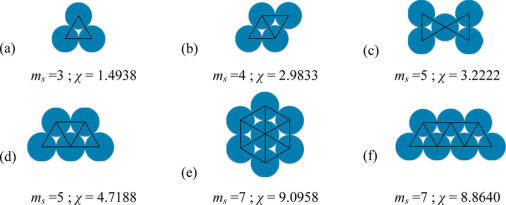
\includegraphics[scale=0.9]{Figures/mullergeo.jpg}
	\caption{Values for parameter $\chi$ according to the ring geometry \cite{muller2017}}
	\label{ringqsi}
\end{figure}

\subsubsection{Combining rules for the intermolecular potential parameters}
\citeonline{lafitte2013} also suggested mixing rules for the potential parameters based on Lorentz-Berthelot combining rules \cite{rowlinson}:
\begin{equation}
\sigma_{ij} =\frac{\sigma{ii}+\sigma{jj}}{2}
\label{eqn:sigmamix}
\end{equation}
\begin{equation}
\lambda_{k,ij} -3 =\sqrt{(\lambda_{k,ii}-3)(\lambda_{k,jj}-3)} , k=r,a
\label{eqn:lambdamix}
\end{equation}
\begin{equation}
\epsilon_{ij} =(1-k_{ij})\frac{\sqrt{\sigma_{ii}^{3}\sigma_{jj}^{3}}}{\sigma_{ij}^{3}}\sqrt{\epsilon_{ii}\epsilon_{jj}}
\label{eqn:epsmix}
\end{equation}

The $k_{ij}$ is a binary interaction parameter to correct the deviations of the Lorentz-Berthelot rule for chemically distinct compounds. This parameter can be fitted to experimental data or pseudo experimental data.


\subsection{Parameter Estimation for the SAFT-$\gamma$ Mie Force Field}\label{parsaft}

The SAFT-$\gamma$ Mie Force Field uses a coarse graining top down methodology in its parameterization. This methodology aims to obtain the intermolecular parameters from macroscopic experimental data such as fluid-phase equilibrium or interfacial tension data. The idea is that the force field  parameters estimated with the SAFT-VR Mie EoS can be used on molecular simulations since both the equation of state and the force field use the same explicit intermolecular potential model (Mie potential). This correspondence between models has already been seen for a variety of fluids in which this force field was parameterized. This success in the representation of the properties of real fluids can be imputed to the degrees of freedom of Mie Potential \cite{herdes2015}. Furthermore, this flexibility provides the exploration of a very large parameter space without using an iterative simulation scheme \cite{avendano2011}. 

Each substance has initially five parameters to be estimated ($m_s$,$\sigma$,$\epsilon$,$\lambda_{r}$ and $\lambda_{a}$) according to Eq. \eqref{eqn:miepotential}. The number of segments are usually fixed in an integer value since each segment represents one pseudo atom. The attractive parameter is generally  fixed due to its  high correlation with the repulsive parameter. Usually, the parameter is fixed in the London value of 6, which is a good representation of the dispersion scale of most simple fluids that don't have strong polar interactions \cite{ramrattan2015,herdes2015}. There are two strategies to obtain the parameters: one is by fitting the Saft-Vr Mie EoS to experimental data as vapor pressure and liquid density and the other one is using correspondent state parametrization. The first, generally, minimizes the following unweighted least-squares objective function:

\begin{equation}
\begin{aligned}
\min\limits_{\sigma,\epsilon,\lambda_{r}} F_{obj}(\sigma,\epsilon,\lambda_{r})= \sum_{i=1}^{N_{p}} \left(\frac{P_{v}^{SAFT}(T_{i},\sigma,\epsilon,\lambda_{r})-P_{v}^{exp}(T_{i})}{P_{v}^{exp}(T_{i})} \right)^2 +\\
\sum_{i=1}^{N_{p}} \left(\frac{\rho_{l}^{SAFT}(T_{i},\sigma,\epsilon,\lambda_{r})-\rho_{l}^{exp}(T_{i})}{\rho_{l}^{exp}(T_{i})} \right)^2
\end{aligned}
\label{eqn:fobj}
\end{equation}
where $N_{p}$ is the number of experimental points, $P_{v}$ is the vapor pressure and $\rho_{l}$ is the saturated liquid density. Another properties that can be used in the estimation are superficial tension and speed of sound. The multiple parameters of the model make it necessary the use of a wide range of experimental data since multiple solutions may be found for the fit. Therefore, one needs to be careful in deciding the level of coarse graining (i.e. the parameter $m_{s}$) and the subsequent parameter space that will not result in some physical inconsistencies such as a premature freezing fluid.

\citeonline{lafitte2012} suggested that two corrections factors ($c_{\sigma}$ and $c_{\epsilon}$) should be estimated with simulation data when using Eq. \eqref{eqn:aringlafitte} for the ring contribution. They are related to the EoS parameters by scaled parameters:

\begin{equation}
\sigma^{scaled} = c_{\sigma}\sigma^{SAFT}
\label{eqn:csigma}
\end{equation}
\begin{equation}
\epsilon^{scaled} = c_{\epsilon}\epsilon^{SAFT}
\label{eqn:ceps}
\end{equation}

According to \citeonline{lafitte2012}, these corrections are necessary because the approximations employed in the EoS theory generate discrepancies between molecular simulations and the EoS for ring molecules modeled with Eq. \eqref{eqn:aringlafitte}. The objective function for this estimation is given by:

\begin{equation}
\begin{split}
\min\limits_{c_{\sigma},c_{\epsilon}} F_{obj}(c_{\sigma},c_{\epsilon})= \sum_{i=1}^{N_{p}} \left(\frac{P_{v}^{sim}(T_{i},\sigma^{SAFT},\epsilon^{SAFT})-P_{v}^{SAFT}(T_{i},\sigma^{scaled},\epsilon^{scaled})}{P_{v}^{sim}(T_{i},\sigma^{SAFT},\epsilon^{SAFT})} \right)^2 + \\
\sum_{i=1}^{N_{p}} \left(\frac{\rho_{liq}^{sim}(T_{i},\sigma^{SAFT},\epsilon^{SAFT})-\rho_{liq}^{SAFT}(T_{i},\sigma^{scaled},\epsilon^{scaled})}{\rho_{liq}^{sim}(T_{i},\sigma^{SAFT},\epsilon^{SAFT})} \right)^2
\end{split}
\label{eqn:fobjla}
\end{equation}

The repulsive parameter is maintained in the value found on the minimization of Eq. \eqref{eqn:fobj}. The refined values for $\sigma$ and $\epsilon$ are:

\begin{equation}
\sigma^{sim} = \sigma^{SAFT}/c_{\sigma}
\label{eqn:simsigma}
\end{equation}

\begin{equation}
\epsilon^{sim} = \epsilon^{SAFT}/c_{\epsilon}
\label{eqn:simeps}
\end{equation}

It is interesting to point out that this new parameterization is not necessary when using Eq. \eqref{eqn:aringmuller} as the ring contribution. The other method to obtain the force field parameters is the correspondent state parametrization \cite{mejia2014}. This method considers that the unweighted volume average of the attractive contribution to the Mie intermolecular potential,$a_{1}$, is a mean field approximation:

\begin{equation}
a_{1} = 2\pi\rho\sigma^{3}\epsilon\alpha
\label{eqn:a1corres}
\end{equation}

The van der Waals constant, $\alpha$, considering $ \lambda_{a} = 6$ is related by the Mie exponents by:

\begin{equation}
\alpha = \frac{1}{\epsilon\sigma^{3	}} \int_{\sigma}^{\infty} \phi(r)r^{2}dr = \frac{\lambda_{r}}{3(\lambda_{r}-3)}\left(\frac{\lambda_r}{6}\right)^{6/(\lambda_{r} - 6)}  
\label{eqn:alpha}
\end{equation}

The parameterization in this method starts by using the experimental acentric factor, $\omega$, for each molecule with a fixed value of $ m_{s}$ to obtain the value of the repulsive exponent with the following Padé series:

\begin{equation}
\lambda_{r} = \frac{\sum_{i=0} a_{i}\omega^{i}}{1+\sum_{i=1} b_{i}\omega^{i}}   
\label{eqn:lambdaco}
\end{equation}

$a_{i}$ and $b_{i}$ are dependent parameters of the number of segments and a table with their values is presented in the original paper \cite{mejia2014}. The van der Waals constant can be found substituting $\lambda_{r}$ into Eq. \eqref{eqn:alpha}. The reduced critical potential $T_{c}^{*}$ is related to $\alpha$ by a Padé series: 

\begin{equation}
T_{c}^{*} = \frac{\sum_{i=0} c_{i}\alpha^{i}}{1+\sum_{i=1} d_{i}\alpha^{i}}   
\label{eqn:tc}
\end{equation}

The values of $c_{i}$ and $d_{i}$ are also available in the original paper. The reduced temperature of the equation above is used in conjunction with the experimental critical temperature, $ T_{c}$, to find the energy parameter with the relation below:

\begin{equation}
T_{c}^{*} = \frac{\kappa_{b}T_{c}}{\epsilon}   
\label{eqn:epscorre}
\end{equation}

The diameter parameter, however, is not obtained with the critical properties, but with the reduced liquid density,$\rho_{T_{r}=0.7}$, at the reduced temperature ,$T_{r}$, of $0.7$. This density is also obtained with a Padé series using parameters by \citeonline{mejia2014}:

\begin{equation}
\rho_{T_{r}=0.7}^{*} = \frac{\sum_{i=0} j_{i}\alpha^{i}}{1+\sum_{i=1} k_{i}\alpha^{i}} 
\label{eqn:denscorre}
\end{equation}

The relation among the equation above, $\sigma$ and the experimental density is given by:

\begin{equation}
\rho_{T_{r}=0.7}^{*} = \rho_{T_{r}=0.7}\sigma^{3}N_{av}   
\label{eqn:sigmacorre}
\end{equation}
where $N_{av}$ is The Avogadro number. This correspondent state method has the advantage of only requiring critical data, which is available for a great range of fluids, and liquid density data. The parameters found with this strategy are available at an online database \cite{ervik2016}.     

The binary interaction parameter $k_{ij}$ of Eq. \eqref{eqn:epsmix} is necessary to adjust the mixture behavior of chemically distinct components. Normally, it is estimated minimizing the difference between experimental binary vapor liquid equilibrium or interfacial tension data and the SAFT-VR Mie EoS output data \cite{muller2017,lobanova2016}. The objective function is similar to: 

\begin{equation}
\begin{aligned}
\min\limits_{k_{ij}} F_{obj}(k_{ij})= \sum_{k=1}^{N_{p}} \left(\frac{P_{v}^{SAFT}(T_{k},x,k_{ij})-P_{v}^{exp}(T_{k},x)}{P_{v}^{exp}(T_{k},x)} \right)^2 +\\
\sum_{k=1}^{N_{p}} \left(\frac{\rho_{l}^{SAFT}(T_{k},x,k_{ij})-\rho_{l}^{exp}(T_{i})}{\rho_{l}^{exp}(T_{i})} \right)^2
\end{aligned}
\label{eqn:fobjmix}
\end{equation}

However, \citeonline{ervik20162} used molecular simulation results to fit the parameter to the superficial tension data. The strategy followed by them was to do simulations in three values of $k_{ij}$ first and, after, they refined the parameter until a value in good agreement with the experimental data was found. 

\section{Solvation Free Energies Simulations Based on Molecular Dynamics}
% background topics

Free energies can be expressed as averages over ensembles of atomic configurations generated using Monte Carlo or molecular dynamics techniques. In the canonical ensemble, the free energy is given by:  

\begin{equation}
\label{eq:fcano}
\begin{aligned}
F(N,V,T) = -\kappa_{b}T ln Q(N,V,T)
\end{aligned}
\end{equation}
where $Q(N,V,T))$ is the partition function of the canonical ensemble:

\begin{equation}
\label{eq:partican}
\begin{aligned}
Q(N,V,T) = \int d^{n}p d^{n}r \exp \left[ -\beta \left( \sum_{i=1}^{N}\dfrac{p_{i}^{2}}{2m_{i}} + U(r_{1},..,r_{n}) \right)
\right]
\end{aligned}
\end{equation}
where $\beta=1/k_{b}T$. Meanwhile, the average over the isothermal-isobaric ensemble gives the Gibbs free energy:

\begin{equation}
\label{eq:fisobari}
\begin{aligned}
G(N,P,T) = -\kappa_{b}T ln \Delta (N,P,T)
\end{aligned}
\end{equation}
where $\Delta (N,P,T)$ is the partition function of the isothermal-isobaric ensemble:

\begin{equation}
\label{eq:partiso}
\begin{aligned}
\Delta (N,P,T) = \frac{1}{V_{0}} \int_{0}^{\infty} dV \int d^{n}p d^{n}r \exp \left[ -\beta \left( \sum_{i=1}^{N}\dfrac{p_{i}^{2}}{2m_{i}} + U(r_{1},..,r_{n}) + PV(r_{1},..,r_{n}) \right) \right]
\end{aligned}
\end{equation}

Evaluating the partition function is a difficult task, but we are interested in calculating the Gibbs free energy difference between two states of a system, that is given by: 

\begin{equation}
\label{eq:dif}
\begin{aligned}
\Delta G_{AB} = G_{B} - G_{A}= -\kappa_{b}T ln \left( \frac{\Delta_{B}}{\Delta_{A}}\right) 
\end{aligned}
\end{equation}

Since the masses of particles in systems 0 and 1 are the same, the moment integrals in the ratio ${\Delta_{B}}/{\Delta_{A}}$ can be simplified into to the ratio of the configuration integrals:

\begin{equation}
\label{eq:partiso}
\begin{aligned}
\dfrac{Z_{B}}{Z_{A}} = \dfrac{\int_{0}^{\infty} dV \int d^{n}r \exp \left[ -\beta \left(U(r_{1},..,r_{n}) + PV(r_{1},..,r_{n}) \right)_{B} \right]}{\int_{0}^{\infty} dV \int d^{n}r \exp \left[ -\beta \left(U(r_{1},..,r_{n}) + PV(r_{1},..,r_{n}) \right)_{A} \right]}
\end{aligned}
\end{equation}

What results in the following equation for the Gibbs free energy difference:

\begin{equation}
\label{eq:dif}
\begin{aligned}
\Delta G_{AB} = G_{B} - G_{A}= -\kappa_{b}T ln \left( \frac{Z_{B}}{Z_{A}}\right)
\end{aligned}
\end{equation}

The Gibbs free energy difference between end states $A$ and $B$ are, more specifically, the difference between the solute alone in the gas phase and the solute interacting with the solvent. In order to these differences be accurate, the states' phase integral must have sufficient overlap  \cite{klimovich}. This can be achieved by calculating the free energy difference between a series of intermediates states. The result of these differences are independent of the path chosen since free energy is a state function. That's why alchemical states (no physical sense) are used to link physical states of interest. The solvation free energy calculations are done through a thermodynamic cycle to gradually insert the solute molecule into the solvent as illustrated in \figref{thermcy}. According to this cycle, the free energy of solvation is expressed as:

\begin{equation}
\label{eq:freesolv}
\begin{aligned}
\Delta G_{solv} = \Delta G_{1 \rightarrow 4} = \Delta G_{1 \rightarrow 2} + \Delta G_{2 \rightarrow 3} + \Delta G_{3 \rightarrow 4}  
\end{aligned}
\end{equation}

\begin{figure}[th]
	\centering
	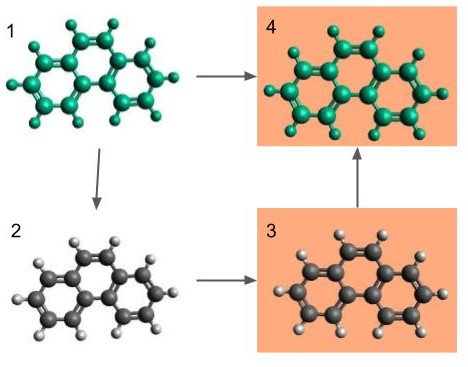
\includegraphics[scale=0.6]{Figures/cicclotermo.jpg}
	\caption{Thermodynamic cycle for solvation free energy calculations with molecular dynamics (Adapted from \citeonline{klimovich})}
	\label{thermcy}
\end{figure}

The solvation free energy between states 1 and 2 in \figref{thermcy} is associated with turning off the molecule's non bonded interactions in the gas phase. The following transformation, $\Delta G_{2 \rightarrow 3}$, is the free energy of moving the non-interacting molecule in the gas phase to the solvent, and is equal to zero since the transformation of a non-interacting molecule doesn't depend on the environment. Lastly, $\Delta G_{3 \rightarrow 4}$ is the free energy required to the non-interaction molecule in the aqueous phase regain its non-bonded interactions.  The solvation free energy calculation can be classified according to the types of non bonded interactions that are turned off in the $1 \rightarrow 2$ and $ 3 \rightarrow 4$ parts of the cycle. If both non-bonded interactions with the environment and internal interactions are turned off, this is an annihilation free energy calculation. Meanwhile, if only non-bonded interactions with the environment are turned off,this is a decoupling free energy calculation. In the later case, $\Delta G_{1 \rightarrow 2} = 0$ and the $\Delta G_{solv} = \Delta G_{3 \rightarrow 4} $. The methods used to carry out these transformations scale the solute charges to zero and then turn off the interactions corresponding to the Lennard Jones potential. In order to carry out the later process, a modified potential with a coupling parameter($\lambda$) is used. Each $\lambda$ represent an alchemical state and, when $\lambda=0$, there is no interaction with the solvent and, when $\lambda=1$, interactions are fully activated. The coupling of the $\lambda$ parameter could be linear, but it could generate numerical problems related to the exponential part of the potential.  That's why the non-linear soft-core scheme \cite{beutler1994} is used to make the potential behave more smoothly in relation to the change of $\lambda$ as can be seem in \figref{fig:SC}. The generalized soft core potential is given by:

\begin{equation}
\label{eq:softcore}
\begin{aligned}
U^{sc}(r) {}=& \lambda\epsilon\dfrac{\lambda_r}{\lambda_r - \lambda_a} \left(\frac{\lambda_r}{\lambda_a} \right)^{\left( \frac{\lambda_a}{\lambda_r - \lambda_a} \right)} \\
& \left\lbrace\dfrac{1}{\left[\alpha(1-\lambda)+ (r/\sigma)^{\lambda_a}\right]^{\lambda_{r}/\lambda_{a}}} - \dfrac{1}{\alpha(1-\lambda)+(r/\sigma)^{\lambda_a}}\right\rbrace
\end{aligned}
\end{equation}
where $\alpha$ is a constant which the value of 0.5 is normally assumed to it,r is the distance the molecules, $\epsilon$ is the depth of the potential well, $\sigma$ is the distance correspondent to a zero intermolecular potential, $\lambda_r$ is the repulsive exponent and $\lambda_a$ is the attractive exponent. Using the Lennard Jones exponents ($\lambda _{r} =12$ and $\lambda _{a} = 6$), Eq. \eqref{eq:softcore} becomes:

\begin{equation}
\label{eq:softcoreLJ}
\begin{aligned}
U_{LJ}^{sc}(r) {}=& 4\lambda\epsilon \left\lbrace\frac{1}{\left[\alpha(1-\lambda)+ (r/\sigma)^{6}\right]^{2}} - \frac{1}{\alpha(1-\lambda)+(r/\sigma)^{6}}\right\rbrace
\end{aligned}
\end{equation}

\begin{figure}[H]
	\centering
	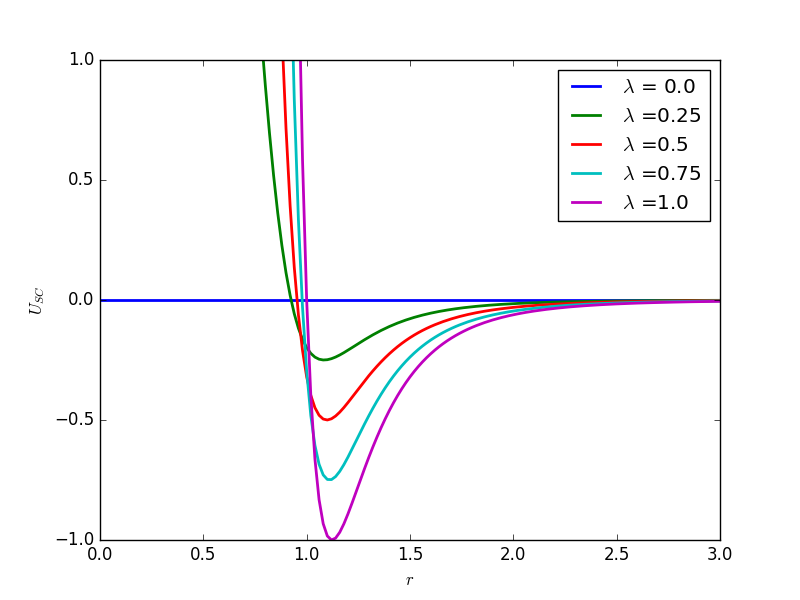
\includegraphics[width=0.9\linewidth]{Figures/SC}
	\caption{Soft-core potential in reduced units.}
	\label{fig:SC}
\end{figure}

The $\Delta G_{3 \rightarrow 4}$ can be then obtained by doing independent simulations in different values of $\lambda$ or by doing expanded ensemble simulations \cite{lyubartsev}, which samples all states in a single simulation. This method allows a faster sampling across the alchemical states, provided that the kinetic barriers are not substantial. The free energies of solvation obtained can then be used to calculate other properties such as the partition coefficient, that is a measure of the partitioning of one solute in two solvents (a and b) at a temperature T:

\begin{equation}
\label{eqn:partcoe}
\log{P}^{a/b} = \frac{\Delta G_{solv}^{a} - \Delta G_{solv}^{b}}{2.303RT}
\end{equation}



\section{Multistate Bennet Acceptance Ratio (MBAR)}\label{mbar}

The MBAR method is a free energy of perturbation based method, the MBAR is equal to the BAR method when the calculations are made between only two states. It proposes an estimator that computes free energies and their uncertainties of all $K$ states  by minimizing the $KxK$ matrix of variances simultaneously for a simulation with $N_{j}$ uncorrelated samples in equilibrium. For each of the ${x_{i,n}}_{n=1}^{N_{i}}$ configurations of i, the following probability distributions is sampled:
\begin{equation}
p_{i}(x) = \frac{q_{i}(x)}{c_{i}}
\end{equation}

\begin{equation}
c_{i} = \int dx q_{i}(x)
\end{equation}
where $q_{i}(x)=exp(-u_{i}(x))$ and $u_{i}$ is the potential energy of each state, defined by $u_{i}= \beta [U_{i}(x)+P_{i}V(x) + \mu _{i}^{T}n(x)]$. Meanwhile, $c_{i}$ is normalization constant.  The free energies are estimated with the ratio of this constant in each state:

\begin{equation}
\Delta f_{ij} = f_{i} - f_{j} = - ln \frac{c_{j}}{c_{i}}  = -ln \frac{\int dx q_{j}(x)}{\int dx q_{i}(x)} 
\end{equation}

\citeonline{mbar} then proposed the following arbitrary function:

\begin{equation}
c_{i} \langle \alpha _{ij} q_{j} \rangle _{i}  =  c_{j} \langle \alpha _{ij} q_{i} \rangle _{j} 
\end{equation}

Using the above equation for every state  K, the relation bellow is obtained:

\begin{equation}
\label{eq:mbar1}
\sum_{j=1}^{K} \frac{\hat{c_{i}}}{N_{i}} \sum_{n=1}^{N_{i}} \alpha _{ij} q_{j} (x_{i,n}) =  \sum_{j=1}^{K} \frac{\hat{c_{j}}}{N_{j}} \sum_{n=1}^{N_{j}} \alpha _{ij} q_{i} (x_{j,n})
\end{equation}

\citeonline{mbar} suggestedd the following equation for $\alpha _{ij}$ in order to decrease the variance:

\begin{equation}
\label{eq:mbar2}
\alpha _{ij} (x) = \frac{N_{j} \hat{c_{i}} ^{-1}}{\sum_{k=1}^{K} N_{k} c_{i} ^{-1} q_{k}(x)}
\end{equation}

Assuming the sampling is carried out following Boltzmann statistics, Eqs. \eqref{eq:mbar1} and \eqref{eq:mbar2} can be rearranged to obtain the free energy estimator that solves self consistently the equation:  

\begin{equation}
\label{eq:mbar}
\begin{aligned}
f_{i} = \frac{1}{\beta}ln \sum_{k=1}^{K} \sum_{n=1}^{N_{k}}
\dfrac{\exp[-\beta u_{i}(x_{kn})]}{\sum_{l=1}^{K} N_{l} \exp[\beta (f_{l} - u_{l}(x_{kn}))]}
\end{aligned}
\end{equation}

The equation above requires the evaluation of the potential energy  of uncorrelated configuration $n$ for all K states ($u_{i}(x_{kn}$) and for all uncorrelated configuration snapshots ($N_{k}$) from state $k$. Free energy changes between states are given then by $\Delta f_{ij} = f_{j} -  f_{i}$. The statistical variance of $S_{ij}^{2} \Delta f_{ij}$ is given by the matrix covariances:

\begin{equation}
\label{eq:varmbar}
\begin{aligned}
s_{ij}^{2} \Delta f_{ij} \equiv cov (-ln \hat{Z_{j}}/\hat{Z_{i}},-ln \hat{Z_{j}}/\hat{Z_{i}})
\end{aligned}
\end{equation}
where $\hat{Z_{j}}$ and $\hat{Z_{i}})$ are the partition functions of states $i$ and $j$. The MBAR method can be considered as limit case of the 
Weighted Histogram Analysis Method (WHAM) \cite{wham} for computing free energies. Eq. \eqref{eq:mbar} becomes equal to the WHAM equations if the histogram width tend to zero. Despite this, the MBAR is still more suited because it doesn't have the bias associated with the discretization  and it allows the calculation of an error estimate.

\section{Expanded Ensemble Method}\label{ee}
%more fundamental 
Instead of doing various simulations in different values of $\lambda$, expanded ensemble simulations \cite{lyubartsev} were developed to allow a non-Boltzmann sampling scheme of different states in only one simulation. In this scheme, the sampling is done by biasing the phase space exploration process with weights not related to the statistical ensemble. The statistical expanded ensemble, $Z^{EE}$, is obtained from the probability distributions correspondent to each $\lambda$, hence $Z^{EE}$ is defined as a sum of sub ensembles $Z_{i}$ in different values of $\lambda$:

\begin{equation}
Z^{EE} = \sum_{i=1}^{N} Z_{i}(\lambda_{i}) exp(\eta_{i})
\label{eqn:ee}
\end{equation}   
where N is the number of alchemical states, $\eta_{i}$ is the arbitrary weight of the sub ensemble at each state and $Z_{i}$ is configuration partition function at state i. For the isothermal-isobaric ensemble, $Z$ is:

\begin{equation}
Z = {\int_{0}^{\infty} dV \int d^{n}r \exp \left[ -\beta \left(U(\lambda, r_{1},..,r_{n}) + PV(r_{1},..,r_{n}) \right) \right]}
\end{equation} 

In solvation free energy calculations with molecular dynamics, $\lambda$ corresponds to the coupling parameter of the soft-core potential (Eq. \ref{eq:softcore}). For molecular dynamic simulations, the sampling of the expanded ensemble is done by performing an arbitrary number of MD  steps followed by a $\lambda$ transition. \citeonline{chodera2011} proved that type of sampling of the expanded ensemble is similar to the Gibbs sampling method \cite{geman1984,liu2002}. Following the Gibbs method, the sampling of the configuration space x for one state $\lambda_{k}$ during the MD steps is done by using the conditional distribution:

\begin{equation}
\pi(x|\lambda_{k}) = \dfrac{\exp[-\beta u(x,\lambda_{k})]}{\int dx \exp [- \beta u(x,\lambda_{k})]}
\label{eqn:rhoee1}
\end{equation} 

Meanwhile, the state transition in the MD simulation uses the following conditional distribution:

\begin{equation}
\pi(\lambda_{k}|x) = \dfrac{\exp[-\beta u(x,\lambda_{k}) + \eta_{k}]}{ \sum_{k=1}^{K} \exp [- \beta u(x,\lambda_{k})+ \eta_{k}]}
\label{eqn:rhoee2}
\end{equation} 
where $u(x,\lambda_{k}) = U(x,\lambda_{k}) + PV(x,\lambda_{k})$ is the reduced potential function for the NPT ensemble. There are a variety of acceptance schemes to do the expanded sampling using Eq. \eqref{eqn:rhoee2}, but \citeonline{chodera2011} suggested that the independence sampling \cite{liu2002} is the best strategy to increase the number of uncorrelated configurations. The implementation suggested by them updates the state index from $i$ to $j$ by first generating a uniform random number $R$ on the interval $[0,1)$ and then selecting the smallest new value of $j$ that satisfies  the relation below:

\begin{equation}
R < \sum_{i=1}^{j} \pi(\lambda_{i}|x) 
\label{eqn:relee2}
\end{equation} 

The sampling strategy above depends on the weights in order to assure an adequate sampling of the states. If there isn't a sufficient number of states sampled, the expanded ensemble becomes deficient in obtaining input data to estimate free energy differences with the methods exposed in Chapter 2. The weights can be calculated following the flat-histogram approach \cite{bernd1992,bernd1993,dayal2004}. This strategy aims to obtain adequate sampling by assuring that all the states have an equal number of samples, i.e. the ratio of the probability of sampling state ($\pi_{i}$) to the probability of sampling state $j$ ($\pi_{j}$) is equal to one. Given that $\pi_{i}$ has the following equation:

\begin{equation}
\pi_{i} = \dfrac{Z_{i}(\lambda_{i}) exp(\eta_{i})}{Z^{EE}} 
\label{eqn:wei1}
\end{equation} 
and using Eqs. \ref{eq:dif} and \ref {eq:partiso}, the following relation can be obtained for $\pi_{i}/\pi_{j}=1$:

\begin{equation}
(\eta_{i} - \eta_{j}) = \beta(G_i-G_j)
\label{eqn:weight}
\end{equation}

Eq. \eqref{eqn:weight} is solved iteratively with trial simulations. For the first simulation, the values of $\eta$ are chosen or set to zero and the histogram of the states visited is obtained. With this histogram, it is possible to estimate the free energy differences and, since the weights are related to the free energies by Eq. \eqref{eqn:weight}, the next values of $\eta$ can be calculated. This iteration goes on until a uniform distribution is secured. The weights found are then used in a longer simulation to obtain the final solvation free energy differences.

The choice of the $\lambda$ set correspondent to overlapping alchemical states are crucial to acquire accurate energy differences. In this work, the method chosen to obtain the optimal stage of the $\lambda$ domain is the one developed by \citeonline{escobedo2007} with basis in the study of  \citeonline{trebst2004}. This method targets "bottlenecks" in the simulation. It does that by optimizing $\lambda$ through the minimization of the number of round trips per CPU time between the lowest $\lambda$ ($=0$) and highest $\lambda$ ($=1$). This is specifically done by maximizing the steady-state stream $\phi$ of the simulation, which "walks" among the values of $\lambda$. This stream is estimated from Fick's diffusion type of law:

\begin{equation}
\phi = D(\Lambda) \Pi (\Lambda) \dfrac{dx(\Lambda)}{d \Lambda}
\label{eqn:stream}
\end{equation}

In the equation above, $\Lambda$ is the actual continue value of the coupling parameter. This continue function of $\lambda s$ is obtained by interpolating the $\lambda$ set linearly. $D(\Lambda)$ is the diffusivity at  state $\Lambda$ and $x(\Lambda)$ is the fraction of times that the trial simulation at state $\Lambda_{i}$ has most recently visited the state $\lambda=1$ as opposed to state $\lambda=0$. The derivative ${dx(\Lambda)}/{d \Lambda}$ is approximated with the central finite differences method. Finally, $\Pi (\Lambda)$ is the probability of visiting $\Lambda$:

\begin{equation}
\Pi (\Lambda) = \dfrac{C^{'} \bar{\Pi} (\lambda)}{\Lambda_{i+1} - \Lambda_{i}}
\label{eqn:plambda}
\end{equation}

The $C^{'} $ term in the equation above represents a constant and $\bar{\Pi} (\lambda)$ is the arithmetic average of visiting the $\Lambda$ states:

\begin{equation}
\bar{\Pi} (\lambda) = \dfrac{\pi_{i+1} - \pi_{i}}{2}
\label{eqn:barplambda}
\end{equation}

The $\phi$ is maximum when the probability $\Pi^{'}(\Lambda_{i})$ is proportional to $1/\sqrt{D(\Lambda)}$. With that information, it is possible to estimate the diffusivity using one trial simulation with the following equation:

\begin{equation}
D(\Lambda) = \dfrac{\Lambda_{i+1} - \Lambda_{i}}{\bar{\Pi} (\lambda) {dx(\Lambda)}/{d \Lambda}}
\label{eqn:diff}
\end{equation}

Hence, we can calculate $\bar{\Pi} $ and, consequently, the cumulative probability, which is used to obtain the new $\lambda$ states:

\begin{equation}
\Phi = \int_{\lambda =0}^{\lambda =1} \Pi^{'}(\Lambda_{i}) d \Lambda = \dfrac{i}{K}
\label{eqn:cumfun}
\end{equation}
where, $K$ is the total number of $\lambda$ states. 

\section{Gibbs Ensemble Monte Carlo (GEMC)}\label{gemc}

The Monte Carlo (MC) approach is another method for generating atomic trajectories in order to obtain macroscopic properties. The trajectories are obtained stochastically, unlike the molecular dynamics approach. The positions are evolved by random moves (MC steps) or perturbations obtained with the Metropolis method \cite{1953JChPh..21.1087M}, hence the positions are not predictable from the set of initial positions. The Metropolis method is a Markov process, that is a stochastic process in which the configurations change randomly with time and have no memories of the previous configurations. The random move is constructed in such way that the probability of visiting a particular point $r^{N}$ is proportional to the Boltzmann factor ($exp[-\beta U(r^{N})]$) \cite{frenkel}. The construction of a  MC according to \citeonline{1953JChPh..21.1087M} can be briefly summed up in:

1. Pick a random particle, and calculate its energy $U(r^{N})$.

2. Perturb the particle by randomly displacing  its configuration, $r' = r +\Delta$. Where $\Delta$ is a perturbation chose from a defined interval of maximum displacement ($[- \delta _{max},\delta _{max}]$). Calculate the energy with the ne positions $U(r'^{N})$.

3. Accept the move from $r^{N}$ to $r'^{N}$ with the probability:
\begin{equation}
	acc_{A \rightarrow B} = min(1,exp[-\beta U(r'^{N}) + \beta U(r^{N}) ])
\end{equation}

The  Monte Carlo simulations are interesting when we need to calculate properties in different thermodynamic ensembles, such as the Gibbs Ensemble \cite{papa1987}. This ensemble  is used to study phase coexistence with simultaneous Monte Carlo (MC) simulations of two boxes,  representing a two phase system, with periodic conditions. The boxes exchange molecules, energy and volume between them. Equilibrium is obtained through MC steps that consist of translation and rotation moves, volume exchange moves and randomly exchanges of molecules between the boxes. For the phase equilibrium of multi-component systems,the GEMC simulations should be carried out at the NPT (constant number of particles, pressure and temperature) ensemble to obey the requirement of an additional degree of freedom for mixtures. Meanwhile, the simulation of single component systems is carried out at constant number of particles, temperature and volume (NVT) since the two phase region would be a line for this system at constant pressure and temperature. The constant volume GEMC ensemble is rigorously equivalent to the canonical ensemble in the thermodynamic limit as demonstrated by \citeonline{frenkel}. The partition function of the GEMC-NVT ensemble is obtained considering that the particles in both boxes are subjected to the same intermolecular interactions. Also, the boxes’ volumes and number of particles ($N_{1}$,$N_{2}$,$V_{1}$ and $V_{2}$) can vary while the total volume ($V$) and total number of particles ($N$) remain constant ($N = N_{1} + N_{2}$,$V = V_{1} + V_{2}$):

\begin{equation}
\begin{aligned}
Q(NVT) {} \equiv & \sum_{N_{1}}^{N} \dfrac{1}{V \Lambda ^{3N} N_{1}!(N-N_{1})!} \int_{0}^{V} dV_{1} V_{1}^{N_{1}} V_{2}^{N_{2}} \int dx_{1}^{N_{1}} \exp[-\beta U(x_{1}^{N_{1}})] \\
& \int dx_{2}^{N_{2}} \exp[-\beta U(x_{2}^{N_{2}})]
\end{aligned}
\label{eqn:gepart}
\end{equation}

In order to define the acceptance rules for the MC moves, it is necessary to know the probability of finding the configuration with $N_{1}$ particles in box 1 with volume $V_{1}$ and positions $x_{1}^{N_{1}}$ and $x_{2}^{N_{2}}$. This probability is given by:

\begin{equation}
\pi(x_{1}^{N_{1}},x_{2}^{N_{2}},N_{1},N_{2},V_{1},V_{2}) \propto \dfrac{V_{1}^{N_{1}}V_{2}^{N_{2}}}{N_{1}!N_{2}!} \exp[-\beta U(x_{1}^{N_{1}}) -\beta U(x_{2}^{N_{2}})]
\label{eqn:geprob}
\end{equation}

The acceptance criterion for the translation and rotation moves of configuration A	to B is similar to the conventional NVT MC ensembles and is equal to:

\begin{equation}
acc_{A \rightarrow B} = \min(1,\exp[-\beta U(x_{A}^{N_{1}}) -\beta U(x_{B}^{N_{1}})])
\label{eqn:drprob}
\end{equation} 

The exchange volume moves happen by exchanging an amount $\Delta V$ between the boxes to achieve pressure equilibrium. $\Delta V$ can be chosen from a uniform distribution based on the maximum variation of volume defined ($\delta V_{max}$) with probability $1/\delta V_{max}$. The acceptance rule for these moves is: 

\begin{equation}
acc_{A \rightarrow B} = \min \left(1, \left(\dfrac{V_{1}^{B}}{V_{1}^{A}} \right)^{N_{1}=1} \left( \dfrac{V_{2}^{B}}{V_{2}^{A}} \right)^{N_{2}+1} \exp[-\beta U(x_{A}^{N}) -\beta U(x_{B}^{N})] \right)
\label{vprob}
\end{equation}

Particle exchange moves are carried out to obtain the equality of chemical potential between the boxes. One particle from one box is removed and then added to a random location in the other box. The criteria to accept or reject this type of move is:

\begin{equation}
acc_{A \rightarrow B} = \min \left( 1, \dfrac{N_{1}V_{2}}{N_{2}V_{1}}  \exp[-\beta U(x_{A}^{N}) -\beta U(x_{B}^{N})] \right)
\label{moleprob}
\end{equation}

This method has been widely used to calculate phase equilibrium, but it under performs for the region near the critical point due to large density fluctuations. The GEMC also has a poor performance for dense systems since the particle exchange moves have a low acceptance ratio for these dense systems.  





